\chapter[Programovanie]{Programovanie}
\label{programovanie} % id kapitoly pre prikaz ref

%Zdroj:
%http://compbio.fmph.uniba.sk/vyuka/prog/index.php/2016/17_Programovanie_(2)_v_Jave

\section{Objektovo orientované programovanie}


	Konkrétne veci (kľúčové slová, syntax, etc.) platia pre Javu, v iných jazykoch sa môžu líšť, ofc
	\subsection{Zapúzdrenie}
	Encapsulation: spojenie dát a súvisiaceho kódu.\\
	Trieda väčšinou navonok ukazuje iba vhodne zvolenú časť metód.\\
	Premenné a pomocné metódy sú skryté.\\
	Preto ich je možné meniť bez zmeny kódu využívajúceho triedu.\\
	
	\subsection{Dedičnosť}
		\begin{itemize}
			\item Trieda môže byť podtriedou inej triedy, napr. trieda Pes môže byť podtriedou všeobecnejšej triedy Zviera, vyjadrujeme kľúčovým slovom extends v definícii triedy - class Pes extends Zviera { ... }
			\item vyhneme sa kopírovaniu podobného kódu
			\item Ak máme premennú typu Shape, môže obsahovať referenciu na objekt triedy Shape alebo jej ľubovoľnej podtriedy - môžeme rôzne typy útvarov spracovávať tým istým kódom.

			\item V Jave sa dedí iba od jednej triedy (na rozdiel od napr. C++). Dedenie je však možné viacúrovňovo
			
			\item Všetky triedy sú automaticky potomkami triedy Object. Trieda Object obsahuje metódy (napr. toString()), ktoré môžeme prekryť.
		\end{itemize}

	\subsection{Polymorfizmus}
		Polymorfizmus v programovaní (hlavne pri OOP) je schopnosť funkcií chovať sa rôzne
		\begin{itemize}
			\item Viacero metód s rovnakým menom ale s rôznymi typmi parametrov, ktoré sa mohli rôzne správať (tzv. overloading)

			\item Podtrieda môže prekryť (override) niektoré zdedené metódy, aby sa chovali inak ako v predkovi - pri dedení navyše sa môže funkcia chovať rôzne v rôznych triedach aj keď sa volá rovnako a má rovnaké typy parametrov.
			\item To, ktorá verzia sa zavolá, záleží od toho, akého typu je objekt, nie akého typu je definovaná referencia
		\end{itemize}

	\subsection{Trieda}
	Trieda je údajový typ definovaný užívateľom. Reprezentuje skupinu objektov, ktoré majú spoločné vlastnosti.
	Do definície triedy dávame: Premenné – pomenované kúsky pamäte, ktoré slúžia na uloženie nejakej informácie alebo dátovej položky, u nás sú to premenné r,i. Metódy – funkcie definované v triede, ktoré vykonávajú operácie pre triedu. Metódy väčšinou pracujú s premennými. V príklade sú to GetI(),SetI()…


		\begin{itemize}
			\item Trieda (class) môže obsahovať niekoľko premenných rôznych typov a metódy, ktoré s premennými v objekte niečo robia.
			\item Inštancia triedy alebo aj objekt triedy (instance, object) je konkrétna hodnota daného typu, t.j. kus pamäti s uloženými premennými triedy
			\item Konštruktory sú špeciálne metódy na inicializáciu premenných v triede. (v Jave je garbage collection - objekty bez referencie na ne sú zmazané, v C++ máme aj deštruktory na odstránenie objektu)
		\end{itemize}
	\subsection{Modifikátory prístupu}
	V Jave:
		\begin{itemize}
			\item \textbf{public:} triedy, rozhrania a ich súčasti prístupné odvšadiaľ
			\item \textbf{prázdny:} viditeľnosť len v rámci balíčka (package)
			\item \textbf{protected:} viditeľnosť v triede, jej podtriedach a v rámci balíčka
			\item \textbf{private:} viditeľnosť len v danej triede
		\end{itemize}
	Iné modifikátory:
		\begin{itemize}
		\item \textbf{abstract:} neimplementovaná metóda alebo trieda s neimplementovanými metódami
		\item \textbf{final:}\\
			-ak je trieda final, nedá sa z nej ďalej dediť\\
			-ak je metóda final, nedá sa v podtriede prekryť\\
			-ak je premenná alebo parameter final, ide o konštantu, ktorú nemožno meniť
		\item \textbf{static:}\\
			- statické premenné a metódy sa týkajú celej triedy, nie konkrétnej inštancie\\
			- statické triedy vo vnútri inej triedy nie sú viazané na jej konkrétnu inštanciu
		\end{itemize}
	\subsection{Konštruktory}
		\begin{itemize}
			\item Úlohou konštruktora je správne nainicializovať objekt
			\item Pri dedení si väčšinou každá trieda inicializuje "svoje" premenné
			\item Napr. Shape inicializuje x a y, Circle nechá inicializáciu x a y na Shape a inicializuje radius.
			\item Prvý príkaz v konštruktore môže byť volanie konštruktoru predka, ktorý voláme kľúčovým slovom super (zo superclass, nadtrieda)
		\end{itemize}
	\subsection{Abstraktné triedy a rozhrania}

		\paragraph{Abstraktné metódy a triedy}
		\begin{itemize}
			\item Aby sa metóda chovala v určitej skupine tried polymorfne, musí byť definovaná v ich spoločnej nadtriede, pre ktorú nemusí existovať zmysluplná implementácia
			\item\textbf{Príklad:} môžeme mať metódu area(), ktorá zráta plochu geometrického útvaru vieme zrátať plochu kruhu alebo obdĺžnika, ale čo je plocha všeobecného útvaru? 
			\item Vtedy môžeme označiť metódu v nadtriede ako \textbf{abstraktnú} (neimplementovanú) potom ale celú nadtriedu treba označiť ako abstraktnú, čo znamená, že nemôžeme tvoriť inštancie tejto triedy (také objekty by totiž nevedeli, čo robiť pri volaní area) podtriedy, ak nie sú absktraktné, musia abstraktné metódy z predka implementovať.
		\end{itemize}
		\paragraph{Interface}
		Podobá sa na abstraktnú triedu, ale 
			\begin{itemize}
				\item neobsahuje premenné ani konštruktory, väčšinou ani implementácie metód - ide teda predošetkým o zoznam abstraktných metód, ktoré treba implementovať
				\item slovo abstract netreba uvádzať, je tam implicitne
				\item trieda môže implementovať viacero rozhraní - pripomína "viacnásobnú dedičnosť"
				\item Jeden interface môže rozširovať iný - dopĺňať ho o ďalšie požadované funkciem používame rovnako kľúčove slovo extends
			\end{itemize}

	\subsection{Vnorené triedy(nested classes)}
	TODO


Zatiaľ sme väčšinou vytvárali triedy alebo rozhrania, ktoré boli priamo členmi balíka (neboli obsiahnuté v žiadnej inej triede). Java však od verzie 1.1 podporuje štyri druhy vnorených tried:

statické členské triedy (static member classes)
Statická členská trieda je definovaná ako statický člen nejakej inej triedy. Takáto trieda sa správa ako obyčajná nevnorená trieda ale má prístup k statickým členom triedy do ktorej je vnorená (aj súkromným).
členské triedy (member classes)
Členská trieda je definovaná ako nestatický člen nejakej inej triedy. Takáto trieda je analogická s členskou metódou. Inštancia členskej triedy je vždy spojená s nejakou inštanciou uzatvárajúcej (enclosing) triedy (akoby mala na ňu v sebe referenciu). Členská trieda má prístup ku všetkým (statickým, nestatický, verejným aj súkromným) členským metódam a premenným uzatvárajúcej triedy.
lokálne triedy (local classes)
Lokálna trieda je trieda definovaná v nejakom bloku programu (čiže v nejakej metóde). Tak isto ako lokálna premenná aj lokálna trieda je viditeľná iba v tomto bloku. Aj keď lokálne triedy nie sú členské triedy, tiež sú definované v rámci nejakej uzatvárajúcej triedy. Preto majú prístup ku všetkým (statickým, nestatický, verejným aj súkromným) členským metódam a premenným uzatvárajúcej triedy (ako členské triedy) ale aj ku konštantným lokálnym premenným viditeľným v danom bloku.
anonymné triedy (anonymous classes)
Anonymná trieda je lokálna trieda, ktorá nemá meno. Spája v sebe syntax pre definíciu triedy a vytvorenie jej inštancie. Zatiaľ čo definícia lokálnej triedy je príkaz, definícia a inštancovanie anonymnej triedy je výraz.


Vzhľadom na to, že nie je v tejto oblasti ustálená terminológia môžeme sa stretnúť s rôznym pomenovaním týchto štyroch typov tried:

Statické členské triedy sa tiež nazývajú vnorené triedy.
Členské triedy sa tiež nazávajú vnútorné triedy (inner classes).
Vnútorné triedy môžu byť tiež všetky triedy okrem statických členských tried.
Pod pojmom vnorené alebo vnútorné triedy sa niekedy môžu myslieť všetky štyri možnosti.





		Java umožňuje definovať triedu v inej triede alebo dokonca v metóde
		To umožnuje ju uložiť tam, kde logicky patrí, kde sa používa a prípadne zamedziť prístup iným častiam programu.
		Trieda definovaná v inej triede môže byť statická alebo nestatická
		

		\paragraph{Statická vnorená trieda (static nested class)}

		Správa sa podobne ako keby bola definovaná mimo triedy
		
		public class A {
		   // premenné, metódy
		   public static class B {
		      // premenné, metódy
		   }
		   
		   // použitie v triede A:
		   B objekt = new B();
		}

		// použitie v inej triede:
		A.B objekt = new A.B();


		\paragraph{Vnútorná trieda, t.j. nestatická vnorená trieda (inner class)}

		Inštancie vnútornej triedy majú prístup k premenným vonkajšej triedy
		
		\paragraph{Lokálna trieda (local class)}

		Podobne ako vnútorná trieda, ale definovaná vo vnútri metódy, priamo prístupná (pod svojim menom) len tam
		Ale inštancie sa dajú použiť aj mimo metódy
		V príklade nižšie metóda iterator obsahuje definíciu triedy MyIterator, ktorá implementuje rozhranie Iterator<Integer>
		Metóda iterator vráti objekt triedy MyIterator metóde main a tá ho implicitne použije vo for cykle, aj keď metóda iterator už skončila

		
		\paragraph{Anonymná trieda (anonymous class)}
		Definuje sa v nejakej metóde, pričom sa jej ani nepriradí meno, iba sa vytvorí inštancia
		Tu je metóda iterator z predchádzajúceho príkladu prepísaná s anonymnou triedou:
		    /** Metoda vrati iterator cez pole */
		    public Iterator<Integer> iterator() {
			return new Iterator<Integer>() { // zaciatok anonymnej triedy
			    private int index = 0;  // poloha v poli, priamo inicializovana
			    public Integer next() { 
				index++;
				return array[index-1]; 
			    }
			    public boolean hasNext() {
				return index < array.length;
			    }
			};  // bodkociarka za prikazom return
		    }

		Za príkaz new sme dali meno rozhrania (Iterator<Integer>), za tým prázdne zátvorky pre "konštruktor", potom definíciu triedy a bodkočiarku
		Nie je možné písať konštruktory, ale môžeme inicializovať premenné, napr. private int index = 0;
		Premenné a parametre z metódy v lokálnych a anonymných triedach

		Lokálna alebo anonymná trieda môže používať aj lokálne premenné a parametre metódy, v ktorej sa nachádza
		Ale pozor, iba ak sú definované ako final alebo sa do nich po inicializácii nič nepriradzuje
		Ak však ide o referenciu na objekt alebo pole, obsah poľa resp. premenných opbjektu je možné meniť, nemení sa iba referencia


	\subsection{garbage collection}
		TODO











Viactvarosť (Polymorphism)
Princípy OOP
Vznik
Počas zrodu prvých programovacích jazykov prevládalo procedurálne programovanie, teda vykoná sa nejaká postupnosť výpočtov a to je všetko.

Prvým krokom smerom k objektom bola (ako ináč) programátorská lenivosť. Programátori boli leniví po štrnásty krát písať ten istý kus programu, napríklad kód zásobníka. Namiesto toho by bolo lepšie vytvoriť si nejaký objekt (triedu,jednotku) Zásobník, ktorý by mal nejaké rozhranie (metódy push,pop,isEmpty) oddelené od implementácie.

Keď niekto chcel používať zásobník, stačilo mu pridať si potrebnú knižnicu k programu a vytvoriť si novú inštanciu triedy/jednotky. To malo za následok napríklad aj zjednodušenie programov (hlavne čo sa týka pochopenia, čo program robí) a tým pádom menej chýb.

Postupne sa Objektovo orientované programovanie (OOP) vyvinulo do dnešnej podoby a sformovalo sa niekoľko základných princípov.

Zapúzdrenie (Encapsulation)
Každá trieda (používateľsky definovaný dátový typ, ktorý spája logicky súvisiace členské dáta, členské funkcie a prípadne ďalšie vnorené dátové typy.) by mala mať rozhranie(interface) na komunikáciu s užívateľom. Toto rozhranie – súbor nejakých metód(funkcií) je všetko, čo by mal užívateľ o triede vedieť. Samotná implementácia metód, použité algoritmy a pomocné dátové štruktúry sú užívateľovi neprístupné.

class Stack {
    // verejné rozhranie:
    public Stack(); // konštruktor
    int pop(); // vyberie a vráti horný prvok
    void push(int x); // vhodí prvok x na vrch
    bool isEmpty(); // vráti true, ak je zásobník prázdny
}
// ...
{
    Stack stack = new Stack();
    stack.push(7);
    stack.push(8);
    while(!stack.isEmpty()) System.out.println(stack.pop());
    // 8 7    
}
Všetky premenné triedy, ktoré sú užívateľovi prístupné by tiež mali byť zapuzdrené. Teda prístupné len pomocou funkcií get, set nikdy nie priamo. Dôvody sú dva

Autor objektu sa môže rozhodnúť, že zmení jeho implementáciu, napríklad namiesto poľa v použije spájaný zoznam, alebo miesto reprezentácie bodu cez karteziánske súradnice x,y bude používať dvojicu, smer a vzdialenosť od stredu súradnicovej sústavy. Programátor, ktorý objekt používal správne len skrz interface, nemusí svoj kód meniť a stále mu bude fungovať, zatiaľ čo programátor, ktorý objektu „šahal“ do premenných, môže písať program odznovu.
Objekt si možno potrebuje pri každej manipulácii udržiavať nejaké dodatočné informácie. Napríklad obdĺžnik si možno chce pri každej zmene rozmerov prepočítať svoj obsah, alebo zásobník si možno potrebuje počítať počet prvkov, ktorý sa mení pri každom volaní push a pop. Keby sme však zmenili obdĺžniku rozmery manuálne alebo zásobníku ručne vyhodili najvyšší prvok, dostali by sme sa do nekorektného stavu.
class Rectangle {
    private int w,h,area;
    private refresh(){ 
        area = w*h;
    }
 
    public int getW(){ return w; }
    public void setW(int value) {
        w = value;
        refresh();
    }
    public int getH(){ return h; }
    public void setH(int value) {
        h = value;
        refresh();
    }
    public int getArea{ return area; }
 
}
Ukrývanie dát (Data hiding)
Ako už bolo spomínané, užívateľ nemá prístup k samotnej implementácii tried, rozhranie je od triedy oddelené. Môže to byť aj preto, že autori triedy jej implemenatáciu taja, alebo aby ju mohli meniť, bez toho aby to ovplyvňovalo správanie programov, ktoré metódy používajú.

Samotná implementácia nie je skrytá len pred programátormi, ale aj pred programom samotným. Všetky veci v triedach majú svoj protection level, ktorý určuje kto k nim môže pristupovať. Poznáme 4 – default, public, private, protected.

Rôzne inštancie
Neodmysliteľnou súčasťou objektového programovania je to, že z jednotlivej triedy sa dajú vytvárať inštancie. Keď máme triedu Zásobník, tak si môžeme vytvoriť kľudne aj 1000 zásobníkov, používať ich naraz a nebudú sa vzájomne rušiť. Objekty potom môžeme používať ako normálne premenné.

Netreba zabúdať, že v Jave a C\# sú triedy referenčný typ a teda nové inštancie nevytvárame priraďovaním cez “=“ ale pomocou príkazu new.

class Dvojica { /*...*/ }
//...
{
    Dvojica d1 = new Dvojica(4,7);  // vytvori sa nova instancia
    Dvojica d2 = d1;                // d2 je odkaz na rovnaku instanciu ako d1
    Dvojica d3 = new Dvojica(2,3);  // zasa nova instancia
    d1.prvy = 1;
    System.out.println(d1.prvy + " " + d2.prvy + " " + d3.prvy);
    // 1 1 2
}
Dedičnosť (Inheritance)
Keď sa nám v programe niečo opakuje, náš kód „smrdí“. Preto ak máme dve triedy, ktoré robia približne to isté, tak ich spoločné vlastnosti by sme mali zhrnúť do ich nadtriedy. Ako to funguje?

Každá trieda môže byť potomkom nejakej inej triedy.

v C++ môže byť trieda potomkom ľubovoľného množstva tried
v Jave a C\# trieda môže dediť vlastnosti jednej triedy a ľubovoľného množstva interface (kompletne abstraktná trieda)
Ak je trieda A potomkom triedy B, tak zdedí, všetky jej vlastnosti, premenné, metódy… Ak trieda B mala metódu M, tak aj A bude mať rovnakú metódu, ktorá robí to isté. Navyše, A si môže vytvoriť vlastnú metódu s rovnakým názvom, vykonávať sa bude metóda z najnižšej vrstvy.

Príklad použitia je v časti Polymorfizmus.

Viactvarosť (Polymorphism)
Ak trieda Kruh dedí z triedy Tvar, tak Kruh je Tvar, takže sa tak aj môže tváriť. Podobne aj Štvorec je Tvar.

Takýto pohľad na vec umožňuje ďalšie zjednodušenie programovania. Predstavte si, že programujete nejakú strategickú hru, kde je 20 druhov pozemných jednotiek všetko sú to rôzne triedy, 15 druhov budov a k tomu nejaké letecké a vodné jednotky. Hráč chce poslať nejakú vybratú skupinu jednotiek do boja. Urobíte teraz cca 50 zoznamov na štýl VybratíLukostrelci, VybratíPešiaci, VybratéKone, VybratéPlachetnice…? Asi nie. Jednoduchšie je spraviť jeden zoznam VybratéJednotky, kde vás netrápi, či jednotka je vojak, kôň, jeden typ lukostrelca alebo piaty typ lukostrelca. Každý z nich bude mať implementované metódy pohniSa(kam), útoč(naKoho), stratilSiŽivot(koľko)… a to bude stačiť na obsluhovanie všetkých 50 typov jednotiek bezbolestne.

Niečo takéto je princíp Polymorfizmu, pristupovať ku triede, akoby to bola nejaká z jeho nadtried.





Typový systém

Jazyk C\# používa CTS (spoločný typový systém - definovaný .NET Framework) a nezavádza žiadne ďalšie typy. Vďaka CTS je možné používať knižničné funkcie medzi rôznymi programovacími jazykmi. Tak ako v Jave, existujú dva typy premenných, hodnotové(primitívne) a referenčné.

Operáciám prevádzajúcim hodnotové (primitívne) typy na odpovedajúce objektovo orientované typy sa hovorí boxing. V opačnom smere unboxing.




Hodnotové typy
Premenné, ktoré sú inštanciou hodnotových typov, priamo reprezentujú nejakú hodnotu. Napríklad premenná typu integer zaberá v pamäti 4 byte a obsahuje priamo hodnotu celého čísla. Nemôžu zostať neinicializované. Priradenie jednej premennej druhej znamená fyzické prekopírovanie reprezentácie hodnoty z jedného miesta na druhé. Premenné sú vytvárané na zásobníku(stack). Zo zásobníku sú odstránené akonáhle je ukončený blok kódu, v ktorom sú definované. V jazyku Java sa nazývajú hodnotové typy primitívne.


Referenčné typy
Premenné, ktoré sú inštanciou referenčných typov, neobsahujú priamo samotné hodnoty, ale obsahujú odkaz na miesto v pamäti, kde je hodnota uložená. Referencia môže mať hodnotu null. Na túto hodnotu sú implicitne inicializované a znamená, že neukazujú na žiadny konkrétny objekt. Hodnotu samotnej referencie nemožno získať ani nie je možné s ňou manipulovať. Referencie ukazujú na haldu(heap). Objekty sú v pamäti automaticky sledované a ich životnosť je riadená pomocou Garbage Collection. Nie je nutné ani dovolené ich explicitne odstraňovať. Vzájomné priradenie dvoch referencií spôsobí iba kopírovanie hodnôt odkazov a nie hodnôt samotných objektov.


Výhody použitia referenčných typov
Keďže s referenciami sa nedá manipulovať, nedajú sa posunúť, napr. pripočítaním nejakého čísla, je možné detekovať, na ktoré objekty už nič neukazuje (a teda sa to môže vymazať). Treba však naprogramovať Garbage Collection poriadne, aby dokázal vymazávať aj objekty, ktoré na seba ukazujú cyklicky, ak na nich už program nemá prístup.

Objekty je možné v pamäti presúvať, upratovať a tým umožniť alokáciu väčších kusov pamäte. Keď máme pamäť príliš rozkúskovanú, máme veľké množstvo malých voľných úsekov, nedokážeme alokovať väčší kus pamäte, hoci by sme mali vedieť. V prípade referencií stačí skompaktovať použitú pamäť. Následne môže byť alokácia efektívnejšia, ako v prípade smerníkov. V dnešnej dobe už ani Garbage Collector nie je taký pomalý, ako v minulosti.

Programátor sa nemusí starať o uvoľňovanie pamäte sám, čo má za následok menší počet chýb v programovaní.











\section{Výnimky (exceptions)}

	Ošetrovanie chýb bez požitia výnimiek
	Do návratového kódu funkcie musíme okrem samotnej hodnoty zakomponovať aj ohlasovanie chýb
	Po každom príkaze, ktorý mohol spôsobiť chybu, musíme existenciu chyby otestovať a vyrovnať sa s tým
	Vedie to k neprehľadným programom

Aj ked sa snažíme písať aplikácie bez chýb, a kompilátor sa nám v tom snaží čo najviac pomáhať (napríklad typovou kontrolou), môžu nastať počas behu aplikácie rôzne chybové stavy. Môžeme ich rozdeliť na neočakávané (delenie nulou, pretečenie aritmetickej operácie, indexovanie mimo rozsah poľa, pretypovanie objektu na nekompatibilný typ, otvorenie neexistujúceho súboru, nedostatok diskového priestoru, …) a očakávané (pri čítaní súboru narazíme na jeho koniec, …). Pomocou výnimiek by sa mali ošetrovať iba situácie výnimočné (neočakávané). Ošetrovanie očakávaných situácií pomocou výnimiek nie je vhodné.



	\subsection{vyhodenie výnimky}

Pre vyhodenie výnimky slúži kľúčové slovo throw. Za ním nasleduje objekt triedy Exception alebo od nej odvodenej.


	Počas behu programu môže dôjsť k rôznym chybám a neobvyklým situáciám, napr. neexistujúci súbor, zlý formát súboru, málo pamäte pri alokovaní polí, objektov, adresovanie mimo hraníc poľa, delenie nulou, ...


	\subsection{zachytenie a spracovanie výnimiek (try, catch), finally}

	Využívame konštrukty try a catch.
	Do try bloku dáme príkazy, z ktorých niektorý môže zlyhať.
	Ak niektorý zlyhá a vyhodí výnimku, okamžite sa ukončí vykonávanie bloku try a pokračuje sa blokom catch. V bloku catch túto výnimku spracujeme, v našom prípade len debugovacím výpisom.


	Pokiaľ chceme zachytiť výnimky, ktoré môžu vzniknúť v nejakom bloku kódu, je potrebné tento blok označiť kľúčovým slovom try. Bezprostredne za ním môže ísť bezprostredne po sebe niekoľko blokov označených kľúčovým slovom catch. Ich účelom je zistiť, o aký druh výnimky ide a vykonať príkazy z jej príslúchajúceho bloku catch. Každá výnimka je vlastne objekt, ktorý je potomkom triedy System.Exception (alebo java.lang.Exception). Druh výnimky, ktorú daný catch spracováva sa určí názvom triedy. Potom spracuje všetky výnimky, ktoré sú tejto triedy alebo jej potomkom.

	Keď nastane výnimka v nejakom bloku try sú zvyšné príkazy až do jeho konca preskočené. Potom môžu byť vykonané príkazy z niektorého bloku catch. Ak chceme mať istotu, že sa určitý kód vykoná vždy, nezávisle na tom, či nastala výnimka alebo nie, musíme za posledný catch zadať ešte blok finally. Obyčajne sa blok finally používa na upratanie po operáciách vykonaných pred alebo v rámci bloku try.



Výnimky prechádzajú hierarchiou volaní metód. Ak teda nebude zachytená v tejto metóde, možno bude zachytená v metóde, ktorá ju volala, alebo v … . Pokiaľ by žiadna metóda výnimku nespracovala (ani Main), prejde výnimka až do operačného systému (virtuálneho stroja), ktorý zastaví vykonávanie aplikácie.

Poradie catch blokov je dôležité. Vždy sa vykoná najviac jeden z nich a to prvý, ktorý špecifikuje triedu, ktorá je rodičom alebo priamo triedou vyhodenej výnimky.



	\paragraph{Rozpoznávanie typov výnimiek}
	Možno by náš program mal rôzne reagovať na rôzne typy chýb, napr.:
	Chýbajúci súbor: vypýtať si od užívateľa nové meno súboru
	Zlý formát súboru: ukázať užívateľovi, kde nastala chyba, požiadať ho, aby ju opravil alebo zadal nové meno súboru
	Nedostatok pamäte: program vypíše, že operáciu nie je možné uskutočniť vzhľadom na málo pamäte
	Toto vieme spraviť, lebo výnimky patria do rôznych tried dedených z triedy Exception (prípadne z vyššej triedy Throwable)
	K jednému príkazu try môžeme mať viacero príkazov catch pre rôzne triedy výnimiek, každý chytá tú triedu a jej podtriedy
	Pri danej výnimke sa použije najvrchnejší catch, ktorý sa na ňu hodí
	Po blokoch try a catch môže nasledovať blok finally, ktorý sa vykoná vždy, bez ohľadu na to, či nastala výnimka a či sa nám ju podarilo odchytiť nejakým príkazom catch
	V tomto bloku môžeme napr. pozatvárať otvorené súbory a pod.


	\paragraph{Propagácia a zreťazenie výnimiek}
	Ak vznikne výnimka v príkaze, ktorý nie je vo vnútri try-catch bloku, alebo ak jej typ nie je zachytený žiadnym catch príkazom, hľadá sa ďalší try-catch blok, napr. vo volajúcej metóde
	Ak výnimku nikto nechytí, program skončí s chybovým výpisom zásobníka

	Pri spracovaní výnimky v bloku catch je možné hodiť novú výnimku (trebárs vhodnejšieho typu)
	Metóda musí deklarovať všetky výnimky, ktoré hádže, alebo ktoré v nej môžu vzniknúť a ich nechytá
	Neplatí pre výnimky triedy RuntimeException a jej podtried a pre Throwable, ktoré nie sú výnimka (ale napr. Error)

	\paragraph{finally}
	Blok finally sa vykoná vždy, keď je aj keď nie je výnimka a aj ak sa výnimku nepodarilo chytiť. Slúži na zatváranie súborov a iné upratovacie práce.


Blok finally sa vždy, za všetkých okolností vykoná pred príkazom return, aj keď try blok alebo catch blok obsahuje príkaz return. * Pokiaľ blok finally obsahuje príkaz return, tak tento return prekryje originálny return v try bloku. Napríklad nasledovná funkcia pre n=2 vráti 0.

	\subsection{vlastné triedy výnimiek}
	Výnimku vyhodíme príkazom throw, pričom musíme vytvoriť objekt nejakej vhodnej triedy, ktorá podtriedou Throwable



Ako sme už spomínali, všetky výnimky sú objekty tried odvodených od triedy Exception. Dôvodom pre vytvorenie vlastných výnimiek môže byť doplnenie vlastných informácií odovzdávaných v objekte výnimky alebo jej odlíšenie od ostatných.

	Môžeme si vytvoriť aj vlastnú triedu, ktorá v premenných môže mať uložené podrobnejšie informácie o chybe, ktorá nastala.
	Väčšinou to bude podtrieda triedy Exception




	\subsection{checked a unchecked výnimky}
Jazyk Java rozdeľuje výnimky ešte na dva typy:

Checked výnimky:
sú potomkovia triedy Exception
metódy musia tieto výnimky ošetriť (catch blok) alebo ich označiť ako neošetrené v klauzule throws za názvom metódy
predstavujú neočakávané situácie mimo priamej kontroly programu (napríklad málo miesta na disku, neexistujúci súbor)
Unchecked výnimky:
sú potomkovia triedy RuntimeException? (napríklad IllegalArgumentException?, NullPointerException?, IllegalStateException)
metódy nemusia tieto výnimky ošetriť ani ich uvádzať v klauzule throws za názvom metódy
predstavujú chyby priamo v programe
Aj keď to môže byť trochu zavádzajúce, RuntimeException? je potomok Exception.



\section{Vlákna (threads)}

%https://micro.dcs.fmph.uniba.sk/dokuwiki/sk:dcs:p3:lectures:lecture4:threads

	Moorov zákon, teda pozorovanie, že každý rok a pol sa výpočtová sila integrovaných obvodov zdvojnásobí, pričom cena ostáva konštantná, v posledných rokoch stráca silu - výroba integrovaných obdovov naráža na technické limity. Riešením, ktoré dovoľuje naďalej zvyšovať výkonnosť je paralelizmus. Podstatnou otázkou je, ako paralelizovať.

Možností je viacero:

„rozsekať“ dáta na niekoľko kusov, každý z nich spracovať zvlášť a na záver ich „zlepiť“ (čo však očividne nie je vhodné pre všetky typy dát a algoritmov)
paralelizovať priamo algoritmus (tiež nevhodné pre niektoré algoritmy)
„špekulatívne vykonávanie dopredu“ - predrátať si na dátach všetky operácie, ktoré môže používateľ vykonať (napríklad načítať všetky webstránky, na ktoré boli linky v aktuálne zobrazenej webstránke) a v momente, keď dá príkaz na ich vykonanie (keď užívateľ klikne na konkrétny link) už len zobraziť vopred vykonanú operáciu
Paralelizácia programov je uskutočniteľná pomocou vlákien, tiež nazývaných odľahčenými procesmi.

Rozdiel medzi vláknom a procesom je v tom, že správa zdrojov procesov je prevádzkovaná operačným systémom - ten dáva pozor, aby si procesy navzájom nesiahali do zdrojov, no pri vláknach táto ochrana nie je zabezpečená: to, aby vlákna manipulovali len s im pridelenými zdrojmi, musí zabezpečiť programátor. Jednému procesu môže patriť viacero vlákien. Výhodou vlákien oproti procesom je väčšia rýchlosť (kontrola procesov systémom a ich prepínanie zaberá istý čas).

Procesor dokáže naraz vykonávať len jedno vlákno/proces - aby vznikol dojem súčasného behu viacerých procesov/vlákien, musia sa rýchlo striedať. Striedanie vlákien môže zabezpečovať virtuálny stroj, no môže ho podporovať aj operačný systém. Striedanie vlákien je nepredvídateľné.


Existujú dva spôsoby, ako implementovať vlákna v Jave: dedením od triedy Thread alebo implementáciou rozhrania Runnable
Implementácia rozhrania Runnable sa používa, ak vytváraný objekt musí byť potomkom inej triedy ako Thread, prípadne ak by jediným dôvodom na dedenie od Thread bolo predefinovanie metódy run().



	\subsection{stav vlákna (new, runnable, blocked, waiting, timed\_waiting, terminated)}







	\subsection{životný cyklus vlákna (vytvorenie, spustenie, zastavenie, ...)}

		Nové vlákno vznikne použitím “new T“, kde T je trieda dediaca od Thread (prípadne samotná trieda Thread). Po vytvorení je vlákno v stave NEW. Na inštancii triedy T sa dá následne zavolať len metóda start(), hocičo iné (s výnimkou metódy setDaemon(), o ktorej bude reč nižšie) vyhodí výnimku. Zavolaním metódy start() vlákno prejde zo stavu NEW do stavu pripravené - RUNNABLE: pridelia sa mu systémové zdroje a naplánuje sa pre beh. Vlákno v stave RUNNABLE buď beží, alebo čaká na priradenie procesoru.

		Zo stavu RUNNABLE sa môže dostať do troch rôznych stavov, ktoré sa súhrnne označujú ako nepripravené, a v ktorých sa vláknu neprideľuje procesor, aj keby bol k dispozícii (čo je žiadané, pretože vlákno nemá čo robiť, a zbytočne by plytvalo systémovými prostriedkami počas aktívneho čakania):

		WAITING - vlákno sa doň dostane zavolaním metódy wait(). Do stavu RUNNABLE ho vráti zavolanie metódy notifyAll() iným vláknom, resp. zavolanie metódy notify() iným vláknom a následne vybratie správcom procesov ako to vlákno spomedzi čakajúcich, ktoré bude upovedomené
		TIMED\_WAITING - do tohto stavu sa vlákno dostane na M milisekúnd zavolaním metódy sleep(M). Po uplynutí daného času sa samo „zobudí“ - prejde do stavu RUNNABLE
		BLOCKED - vlákno môže byť blokované vstupno-výstupnými operáciami alebo zámkom (Lock - bude spomínaný ďalej). Z tohto stavu späť do RUNNABLE ho „zobudí“ operačný systém
		Vlákno skončí (prejde do stavu TERMINATED), keď skončí jeho metóda run(). Celý program skončí, keď skončia všetky jeho vlákna, ktoré nie sú démonmi (ako démoni sú označované vlákna, ktoré nebránia Java Virtual Machine v ukončení programu, aj keď bežia, teda vlákna bežiace „na pozadí“. Typickými príkladom je garbage collection. To, či je vlákno démonom, sa dedí (vlákno bude mať prednastavené, že je démonom, ak bolo démonom aj vlákno, čo ho vytvorilo) a dá sa to zmeniť metódou setDaemon() - pozor, len predtým, ako bola volaná metóda start()).

		Na to, v akom stave vlákno je, sa dá spýtať metódou getState(). Tá vracia jednu zo šiestich konštánt spomínaných vyššie (NEW, RUNNABLE, WAITING, TIMED\_WAITING, BLOCKED, TERMINATED). Ďalšia metóda, ktorá sa môže zísť v súvislosti so stavom vlákna je isAlive() - vracia true, ak vlákno už začalo (bola na ňom zavolaná metóda start()) a zároveň neskončilo (neskončila jeho metóda run()), false v opačnom prípade.


	\subsection{plánovanie vlákien (fixed-priority scheduling, yield, time-slicing)}
Priorita a plánovanie vlákien
Priorita vlákna je celé číslo od 1 po 10 (v triede Thread sú definované konštanty MIN\_PRIORITY ako 1, NORM\_PRIORITY ako 5 a MAX\_PRIORITY ako 10, teda väčšie číslo znamená väčšiu prioritu). Priorita sa dedí (podobne ako to, či je vlákno démonom). Zmeniť prioritu vlákna na P je možné jeho metódou setPriority(P), zistiť jeho prioritu metódou getPriority().


Plánovanie vlákien: keďže na väčšine počítačov naraz beží viac vlákien, ako má počítač procesorov, vlákna sa musia vo využívaní procesora striedať (predstavte si počítač, na ktorom by sa nestriedali. Nie len, že by sa nedalo pracovať s viacerými aplikáciami súčasne, navyše ani v rámci jednej aplikácie by nebolo možné vykonávať niekoľko vecí súčasne - vykonanie výpočtovo zložitejšej operácie (napr. doostrenie veľkej fotografie) by na istý čas odstavilo užívateľský interface aplikácie, tá by „zamrzla“. Preto má zmysel robiť aj aplikácie pre počítače s jedným jadrom viacvláknové).

To, kedy bude ktorému vláknu pridelený procesor určuje algoritmus nazývaný plánovač. Java podporuje jednoduchý deterministický plánovač známy ako fixed-priority scheduling. V ľubovoľnom čase, keď je k behu pripravených viacero vlákien, plánovač spomedzi nich vyberie vlákno s najvyššou prioritou. Ak má niekoľko (všetky) vlákna rovnakú najvyššiu prioritu, vyberie ľubovoľné z nich. Vybrané vlákno beží, kým nenastane jedna z nasledujúcich situácii:

skončí sa jeho metóda run()
bežiace vlákno zavolá metódu yield(), čím sa dobrovoľne vzdá procesora a dá možnosť bežať inému vláknu (plánovač si vyberá ktorému)
medzi pripravenými vláknami sa objaví vlákno s vyššou prioritou než má práve bežiace vlákno
Na systémoch podporujúcich time-slicing môže byť beh vlákna prerušený aj vypršením času, ktoré je vláknu pridelené - Java však time-slicing nešpecifikuje, a preto ho systém nemusí implementovať.

Napriek tomuto nie je zaručené, že v ľubovoľnom okamihu beží vlákno s najväčšou prioritou. Plánovač môže pre beh vybrať aj vlákno s nižšou prioritou, aby tým zabránil jeho „vyhladovaniu“ (čo je situácia, keď vlákno nie je schopné získať prístup k zdieľanému prostriedku a nie je schopné tento stav zmeniť).

Z týchto dôvodov nie je možné sa spoliehať na nejaké konkrétne poradie striedania vlákien: priorita môže byť použitá len na zvýšenie efektivity vykonávania vlákien, nie je možné na nej postaviť korektnosť algoritmu.

Sebeckým vláknom (selfish thread) sa označuje vlákno, ktorého beh je vždy zastavený až skončením jeho metódy run() alebo prerušením vláknom s väčšou prioritou. Takéto správanie je sebecké voči vláknam s rovnakou prioritou, ktoré nemajú šancu bežať, kým sebecké vlákno neskončí. Aby vlákno nebolo sebecké, malo by z času na čas zavolať svoju metódu yield() a tým umožniť beh iným vláknam s rovnakou prioritou. Toto samozrejme nie je nutné, ak systém implementuje time-slicing (vtedy systém automaticky preruší vlákno vtedy, keď mu ubehne čas pridelený na beh), avšak keďže time-slicing nie je Javou vyžadovný, tak aplikácie, ktoré sa naň spoliehajú, nie sú prenositeľné.

Príklad: sebecké vlákno


	\subsection{Synchronizácia vlákien (kritické úseky, wait a notify, explicitné zámky a podmienkové premenné)}

Kritické úseky
Ako to funguje?
wait(), notify() a notifyAll()
Explicitné zámky a podmienkové premenné
Synchronizácia vlákien
Dosiaľ sme sa zaoberali len vláknami, ktoré sa nezaujímali o stav a aktivity iných vlákien. Každé vlákno taktiež obsahovalo všetky dáta a metódy potrebné pre svoj beh. Išlo teda o nezávislé asynchrónne vlákna, ktoré sa o seba nijakým spôsobom nestarali.

Problémy môžu nastať, keď vlákna potrebujú pristupovať k zdieľaným prostriedkom, alebo chcú komunikovať.

príklad: Dve vlákna chcú naraz vypisovať do súboru, vlákno A vypisuje reťazec „aa“, vlákno B vypisuje reťazec „bb“. V prípade, že sa nesynchronizujú, nemusí byť výsledkom „aabb“, resp. „bbaa“, ale môže to byť hocičo zmiešané, napr. „abba“ (vláknu A bol pridelený procesor, stihlo do súboru zapísať znak „a“, vzápätí mu vypršal čas, procesor bol pridelený vláknu B, to stihlo zapísať „bb“, následne bol procesor opäť pridelený vláknu A, ktoré dopísalo druhé „a“). Ide o typický príklad race conditions, teda časovej závislosti - výsledok programu závisí od toho, ako budú naplánované vlákna na beh.
príklad: Vlákna komunikujú posielaním si dát - jedno vlákno je producentom, druhé konzumentom. Producent niečo vyrába (dáta, signály) a posiela konzumentovi, ten to prijíma.

	Je žiadúce písať kritické úseky čo najkratšie, a do kučeravých zátvoriek po synchronized uzatvárať len príkazy, ktoré tam nutne musia byť, nech sa zbytočne príkazmi netýkajúcimi sa zdieľaného zdroja neblokuje prístup k danému zdroju iným vláknam. Kľúčové slovo synchronized sa nededí: ak je metóda M v triede T synchronizovaná, tak predefinovaná metóda M v potomkovi triedy T synchronizovaná byť nemusí (samozrejme, môže). Synchronizácia niečo stojí - volanie synchronizovanej metódy je pomalšie ako volanie nesynchronizovanej. Preto synchronizáciu treba používať len v metódach obsahujúcich kritické úseky.

Ako to funguje?
Každému objektu Java pridelí zámok, ktorý uzamkne, keď nejaké vlákno vstúpi do synchronizovanej časti kódu viažúcemu sa k danému objektu. Keď je zámok uzamknutý, žiadne iné vlákno nemôže zavolať vykonať žiaden synchronizovaný kód viažuci sa na ten istý objekt. Pokiaľ sa o to pokúsi, bude blokované až kým pôvodné vlákno neopustí synchronizovanú časť kódu, čím sa zámok odomkne. Vlákno, ktoré objekt uzamklo, však môže volať synchronizované metódy tohto objektu a vykonávať iný synchronizovaný kód uzamknutý vzhľadom na tento objekt (aj rekurzívne).

Zamykanie a odomykanie Java vykonáva automaticky, ako atomickú (nedeliteľnú) operáciu. Vďaka tomu sa vyhneme problémom, ktoré by mohli vzniknúť ako dôsledok race conditions.

Vráťme sa teraz k príkladu producenta a konzumenta - ich činnosti musia byť synchronizované dvoma spôsobmi:

Pristupovať k objektu Storage môže naraz iba jedno vlákno. Rieši sa uzamykaním objektu (synchronizované metódy).
Producent musí oznámiť konzumentovi, že sú pripravené nové dáta a konzument zas musí oznámiť producentovi, že už dáta prečítal a v Storage je voľné miesto pre ďalšie dáta. Rieši sa metódami wait() a notify().
Synchronizovanie producenta a konzumenta



wait(), notify() a notifyAll()
Treba si uvedomiť, že wait() znamená „zaspi a čakaj, kým ťa niečo nezobudí“ a nie „zaspi a čakaj, kým ťa nezobudí práve to, na čo čakáš“. Preto treba wait() volať v cykle: while (!podmienka) wait();

Podobne notify() znamená „upovedom niekoho o niečom“ - náhodne vyberie jedno z čakajúcich vlákien a to zobudí. Preto sa táto metóda používa len pri optimalizácii, keď všetky vlákna čakajú na tú istú podmienku a je jedno, ktoré sa aktivuje. (notifyAll() analogicky znamená „upovedom všetkých o niečom“.)

Keď vlákno čaká na príkaze wait(), odomkne sa zámok ku ktorému wait() patrí, avšak iné objekty uzamknuté týmto vláknom stále ostávajú uzamknuté.

wait(), notify() a notifyAll() sú použiteľné len v kritických úsekoch, mimo nich vyhadzujú výnimku.

notify() a notifyAll() majú len aktuálny účinok, ak nie je žiadne vlákno, ktoré by sa mohlo zobudiť, účinok metódy notify() (resp. notifyAll()) sa neodloží do budúcna, ale zanikne.

Explicitné zámky a podmienkové premenné
Ďalšia možnosť, ako získať výlučný prístup k časti kódu, je pomocou explicitných zámkov. Ich výhodou oproti synchronizovaným metódam je, že sa môžu zamknúť a odomknúť v rôznych častiach kódu (napríklad to nemusí byť v jednej metóde). Na vytvorenie explicitného zámku treba inštancovať triedu, ktorá implementuje rozhranie Lock, napr. ReentrantLock. Zámok sa potom zamkne zavolaním metódy lock() a odomnke metódou unlock(). Keďže zámok sa automaticky neodomyká pri ukončení metódy, je vhodné uzavrieť lock() a unlock() do bloku try/finally, aby zámok neostal zamknutý pri vzniku výnimky, a neblokoval tým ostatné vlákna.

Pokiaľ je potrebné čakať na explicitnom zámku, vytvorí sa podmienková premenná pomocou metódy Lock.newCondition(). Podmienková premenná je inštancia triedy implementujúcej rozhranie Condition. Rozhranie poskytuje metódy await() (čakanie na podmienku, používa sa na mieste, kde by ste pri použití synchronized použili wait()) a signal() (zobudenie vlákien, ktoré čakali pomocou await() na danej podmienkovej premennej - podobné notifyAll()).


Pozor, aj pri použití explicitných zámkov (rovnako ako pri použití synchronized) sa uzamykajú objekty, a nie kód. Teda ten istý kód v bloku synchronized sa teda môže vykonávať pre rôzne objekty (inštancie).

Na jednom objekte môže čakať viacero vlákien, pričom ich čakanie mohlo vzniknúť na rôznych príkazoch wait().

Každý objekt má dve samostatné fronty: v jednej sú vlákna čakajúce na vstup do s týmto objektom synchronizovaného bloku kódu, v druhej vlákna čakajúce na príkaze wait(). Žiadne vlákno nikdy nie je v oboch frontách súčasne (keďže sa nemá ako dostať do oboch front súčasne). Čakajúce vlákna musí aktivovať iné bežiace vlákno. Metóda notifyAll() aktivuje všetky čakajúce vlákna, tj. presunie všetky vlákna z fronty tých, ktoré čakajú na metóde wait() do fronty tých, ktoré čakajú na vstup do synchronizovaného bloku.



\section{Generics}
	\subsection{formálne typové parametre}
	\subsection{parametrizovaný typ}
	\subsection{wildcards}
	\subsection{ohraničené wildcards}
	\subsection{generic methods}

\section{Návrhové vzory: Composite, Strategy}

Jednotlivé triedy odvodené od triedy Compositor predstavujú jednotlivé formátovacie algoritmy. Konkrétna podtrieda triedy Compositor sa odovzdá objektu Composition pri jeho vytvorení.

Zabalenie algoritmu do samostatného objektu je úlohou návrhového vzoru strategy pattern.
	\subsection{Composite}
		\paragraph{Účel}
			 - Skladanie (komponovanie) objektov do stromovej štruktúry, pričom sa pracuje rovnako s jednoduchými a zloženými objektami.

		\paragraph{Motivácia}
		Pri práci so zloženými objektami sa častokrát používajú iné metódy ako pre prácu so základnými objektami (primitívami) a aj jednotlivé primitíva majú rozdielne metódy. Potom však vznikajú problémy pri používaní týchto objektov. Tieto problémy rieši Composite pattern.


		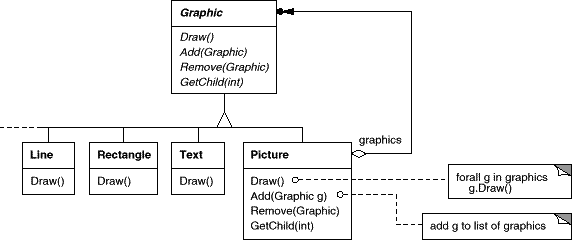
\includegraphics[width=.9\textwidth]{images/programovanie/composite1}

		Graphic je abstraktná trieda pre primitíva ale aj ich kontajnery.


		\paragraph{Použiteľnosť}
		Návrhový vzor Composite sa používa, keď chceme:
			\begin{itemize}
				\item zobraziť hierarchie objektov
				\item pracovať so všetkými objektami v štruktúre jednotne a ignorovať rozdiely medzi primitívnymi objektami a kompozíciami
			\end{itemize}
		\paragraph{Štruktúra}

		:\\
			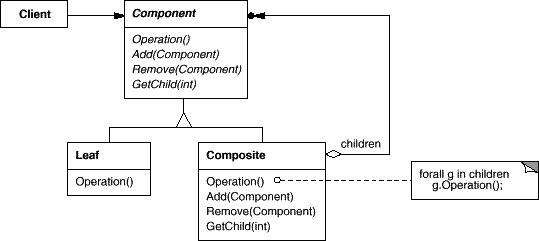
\includegraphics[width=.9\textwidth]{images/programovanie/composite2}

		\paragraph{Účastníci}
			\begin{enumerate}
				\item Component (komponent)\\
				deklaruje rozhranie (interface)\\
				implementuje štandardné správanie\\
				deklaruje rozhranie pre prístup k synom (a aj ich menežovanie)\\
				deklaruje rozhranie pre prístup k rodičovi
				\item Leaf (list)\\
				reprezentuje listový objekt, nemá deti\\
				definuje správanie pre primitívne objekty
				\item Composite (uzol)\\
				definuje správanie pre objekty, ktoré majú synov\\
				uchováva referencie na svojich synov\\
				implementuje operácie pre prácu so synmi
				\item Client (klient)\\
				manipuluje s objektami pomocou rozhrania objektu Component
			\end{enumerate}
		\paragraph{Vzťahy (spolupráca)}
		Client používa rozhranie triedy Component na prácu s objektami. Listy väčšinou vykonávajú požiadavku priamo, uzly ju väčšinou posielajú synom.

		\paragraph{Dôsledky}
		Návrhový vzor Composite:
			\begin{itemize}
				\item definuje hierarchiu tried pozostávajúcu z primitívnych objektov a kompozícií
				\item uľahčuje klientovi manipuláciu s objektami
				\item uľahčuje pridávanie nových typov komponentov
				\item môže spraviť dizajn až príliš všeobecný
				\item môže sa stať, že bude nutné obmedziť nejaké typy komponentov (treba riešiť kontrolami počas behu programu)
			\end{itemize}
		\paragraph{Implementácia}
		Pri implementácii si treba uvedomiť viacero faktov:
			\begin{itemize}
			\item explicitná referencia na rodiča \\
				je potrebná na prechádzanie štruktúrou\\
			 	treba ju starostlivo menežovať (najlepšie iba pri add a remove operáciach v triede Component)
			\item zdieľanie komponentov\\
			pre redukciu priestorovej náročnosti\\
			problém s rodičmi a prechádzaním dokumentu\\
			maximalizovanie rozhrania objektu Component\\
			objekt Component by mal pokrývať celú funkcionalitu\\
			definuje sa všeobecné správanie, ktoré si jednotlivé konkrétne triedy prispôsobia\\
			deklarovanie operácií na prácu so synmi - kde sú definované operácie Add a remove?\\
			ak sú deklarované v triede Component, zachováva sa uniformita, ale stráca sa bezpečnosť (niekto ich môže predefinovať v listoch)\\
			ak sú deklarované v triede Composite, zachováva sa bezpečnosť, ale stráca sa uniformita\\
			\item má Component obsahovať zoznam synov?\\
			áno, ak sú tam definované operácie add a remove\\
			zbytočne to však zaberá miesto v listoch
			\item poradie synov\\
			môže byť dôležité\\
			rieši ho návrhový vzor Iterator
			\item Kešovanie\\
			uchovávanie určitých informácií kvôli urýchleniu (napr. priestor, ktorý zaberá obrázok, aby sa nemusel vykresľovať, ak je neviditeľný)\\
			netreba zabúdať na starostlivé aktualizovanie týchto údajov
			\item Mazanie komponentov\\
			väšinou robí rodič

			\end{itemize}



	\subsection{Strategy}
		\paragraph{Účel}
			Definovať množinu algoritmov, zapúzdriť každý z nich a umožniť ich vzájomnú výmenu.
		\paragraph{Motivacia}
			Ak by sme chceli formátovací algoritmus implementovať priamo v kóde, narazíme na viacero problémov:
				\begin{itemize}
					\item kód je zložitejší (hlavne ak máme viacero algoritmov)
					\item možno nepoužijeme všetky algoritmy, zbytočne ich budeme mať v kóde
					\item ťažko sa pridávajú nové algoritmy
					\item Všetky tieto problémy sa vyriešia definovaním tried, ktoré zapúzdrujú formátovacie algoritmy.\\
				\end{itemize}

				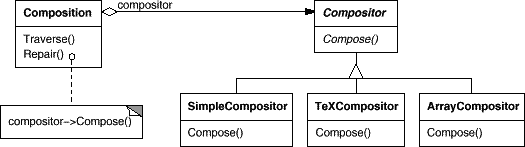
\includegraphics[width=.9\textwidth]{images/programovanie/strategy1}

		Trieda Compositor je abstraktná trieda pre formátovacie algoritmy. Konkrétne algoritmy sú z nej odvodené. SimpleCompositor jednoducho počíta, či už nie sme na konci riadku a ak áno, dá slovo do nového riadku. TeXCompositor robí krajšie (ale časovo náročnejšie) zarovnávanie do riadkov, pričom rovnomerne distribuuje medzery a môže aj podfarbovať text, čo signalizuje, že to ešte nie je zarovnané. ArrayCompositor dá do každého riadku rovnaký počet objektov (napr. ak usporiadavame ikony).


		\paragraph{Použiteľnosť}
			Návrhový vzor Strategy sa používa, ak:
			\begin{itemize}
				\item veľa tried sa líši iba v ich správaní
				\item potrebujeme veľa rôznych druhov algoritmov
				\item algoritmus používa dáta o ktorých nemá Client vedieť
				\item trieda definuje veľa typov správania, ktoré sú implementované pomocou viacnásobných podmienok
			\end{itemize}
		\paragraph{Štruktúra}:\\

			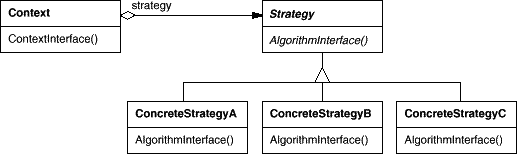
\includegraphics[width=.9\textwidth]{images/programovanie/strategy2}

		\paragraph{Účastníci}
			\begin{enumerate}
				\item Strategy\\
				deklaruje rozhranie
				\item ConcreteStrategy\\
				implementuje algoritmus
				\item Context\\
				je konfigurovaný pomocou ConcreteStrategy objektu\\
				uchováva referenciu na Strategy objekt\\
				môže definovať rozhranie pomocou ktorého Strategy objekt pristupuje k jeho dátam
			\end{enumerate}
		\paragraph{Vzťahy (spolupráca)}
			\begin{itemize}
			\item Strategy a Context spolupracujú pri implementácii algoritmu. Context môže poskytnúť potrebné dáta alebo referenciu na seba.
			\item Context posiela požiadavky od svojich klientov. Klienti zvyčajne vytvoria konkrétnu Strategy triedu, dajú ju Context-u a potom už pracujú výlučne s objektom Context.
			\end{itemize}

		\paragraph{Dôsledky}
			\begin{itemize}
				\item Stratégie definujú triedy súvisiacich algoritmov. Často preto možno využiť dedičnosť pri implementovaní stratégií.
				\item Stratégie sú alternatívou pre dedičnosť (definovanu v triede Context). Mohli by sme aj priamo implementovať formátovací algoritmus v triede Context a modifikovať ho v odvodených triedach, je to však veľmi neprehľadné.
				\item Stratégie eliminujú podmienkové príkazy.
				\item Stratégie môžu ponúkať rôzne implementácie pre rovnaké správanie.
				\item Klient sa musí rozhodovať medzi rôznymi stratégiami, čo ho môže zaťažovať.
				\item Vzniká komunikačná réžia medzi Strategy a Context objektom. Vo väčšine prípadov je však zanedbateľná.
				\item Vzniká väčší počet objektov, možno ich však urobiť bezstavové a zdielať ich.
			\end{itemize}
		\paragraph{Implementácia}:\\
			\textbf{Definovanie rozhraní objektov Strategy a Context.}
				Treba sa zamyslieť nad tým, ako bude najvýhodnejšie odovzdávať potrebné informácie. Context môže poskytnúť potrebné dáta ako parametre metódy Compose, alebo poskytne referenciu na seba a konkrétna stratégia si už potom od neho vypýta to, čo potrebuje. To, ktoré riešenie je výhodnejšie, závisí od konkrétneho problému.

			\textbf{Definovanie Strategy objektu ako dobrovoľného.}
				Trieda Context môže byť naprogramovaná aj tak, že nemusí mať priradenú žiadnu stratégiu (t.j. pri vytváraní objektu typu Context sa mu nepriradí žiadna stratégia). V tomto prípade sa potom vykoná preddefinované správanie. Výhodou je, že klienti nie sú zaťažovaní výberom stratégie, ak nechcú.


\section{Návrhové vzory: Decorator, Abstract Factory}
	\subsection{Decorator}
		
		\paragraph{Účel: }
			Dynamicky pridať ďalšiu funkcionalitu objektu. Decorator predstavuje oproti dedeniu pružnejší spôsob pre rozšírenie funkcionality.

		\paragraph{Ďalšie pomenovania: }
				Wrapper

		\paragraph{Motivácia}
			Niekedy chceme pridať funkcionalitu jednotlivým objektom a nie celej triede. Napr. pri pridaní posuvnej lišty a okraju pre vizuálne komponenty.

			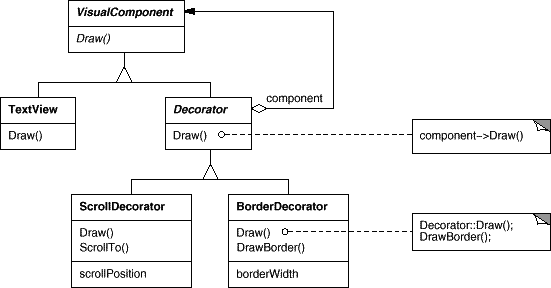
\includegraphics[width=.9\textwidth]{images/programovanie/decorator1}

		\paragraph{Použiteľnosť}
			\begin{itemize}
				\item na pridanie funkcionality pre jednotlivé objekty dynamicky a transparentne (t.j. bez ovplyvnenia ostatných objektov)
				\item na pridanie funkcionality, ktorá je voliteľná
				\item ak rozšírenie funkcionality pomocou dedenia je nepraktické; ak napr. máme veľa typov rozšírení a tak by nám exponenciálne narastal počet odvodených tried
			\end{itemize}
		\paragraph{Štruktúra}:\\


		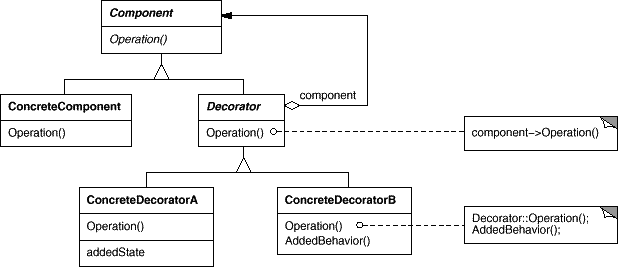
\includegraphics[width=.9\textwidth]{images/programovanie/decorator2}
		
		\paragraph{Účastníci}
			\begin{enumerate}
				\item Component\\
				deklaruje rozhranie (interface) objektov, ktoré môžu mať dynamicky pridávanú funkcionalitu
				\item ConcreteComponent\\
				deklaruje objekt, ktorému chceme pridávať funkcionalitu (konkrétny komponent, napríklad TextView)
				\item Decorator\\
				uchováva referenciu na objekt typu Component (alebo jeho potomka), ktorému pridáva funkcionalitu; definuje rozhranie, ktoré zodpovedá rozhraniu objektu Component
				\item ConcreteDecorator\\
				pridáva konkrétnu funkcionalitu objektu typu Component, alebo jeho potomkovi (konkrétny dekorátor, napríklad ScrollDecorator, BorderDecorator)
			\end{enumerate}
		
		\paragraph{Vzťahy (spolupráca)}
		Decorator posiela väčšinu požiadaviek priamo objektu Component, niekedy však môže predtým alebo potom vykonať aj svoju vlastnú funkcionalitu.

		\paragraph{Dôsledky}:\\
			\textbf{Návrhový vzor Decorator má nasledovné dve výhody:}
			\begin{itemize}
				\item Je viac flexibilnejší ako dedičnosť. Decorator pridáva funkcionalitu za behu (pri dedičnosti by sme museli vytvoriť nový objekt), dovoľuje ľubovoľne kombinovať pridanú funkcionalitu (v poradí, aké potrebujeme), pričom môžeme aj dvakrát pridať tú istú funkcionalitu (dvojitý rámik).
				\item Obmedzuje vytváranie zbytočne zložitých objektov. Decorator ponúka prístup plať iba za to, čo využívaš. Namiesto možnosti podporovať všetky možné funkcionality vo veľkej konfigurovateľnej triede definuje radšej jednoduchú triedu, ktorej pridáva funkcionalitu pomocou objektov Decorator. Výsledkom toho je, že aplikácia nemusí platiť za funkcionalitu, ktorú nepoužíva. Navyše sa ľahko definujú nové typy dekorátorov nezávisle na triedach, ktorým pridávajú funkcionalitu.
			\end{itemize}

			\textbf{Návrhový vzor Decorator má nasledovné dve nevýhody:}
				\begin{itemize}
					\item Decorator aj jeho Component nie sú identické. Hoci Decorator sa správa ako transparentný uzáver, v skutočnosti to nie je objekt Component, čo môže spôsobovať problémy, keď sa spoliehame na identitu objektu.
					\item Pri použití tohoto návrhového vzoru vzniká počas behu programu veľa malých objektov, ktoré častokrát vyzerajú rovnako, môžu sa líšiť iba ich vzájomným poprepájaním. Toto môže robiť problém pri debugovaní ľuďom, ktorí systém nepochopili.
				\end{itemize}
			\paragraph{Implementácia}:\\
				Pri implementácii si treba uvedomiť viacero faktov:
				\begin{itemize}
					\item Prispôsobenie rozhraní.\\
					Rozhranie objektu Decorator musí zodpovedať rozhraniu objektu, ktorému funkcionalitu pridáva.
					\item Vynechanie abstraktnej triedy Decorator.\\
					Ak chceme pridať iba jednu jedinú funkcionalitu, môžeme vynechať abstraktnú triedu Decorator a môžme priamo pracovať s nejakou triedou ConcreteDecorator. Toto riešenie je vhodné najmä ak nemôžeme rozširovanú triedu modifikovať a tak do nej priamo doplniť požadovanú jednu funkcionalitu.

					\item Ľahká trieda Component.\\
					V abstraktnej triede Component by sme sa mali zamerať na zadefinovanie iba potrebných metód. Nemala by obsahovať zbytočné metódy a ani premenné, aby nezaťažovala triedu Decorator (a ani ostatné od nej odvodené triedy). Ak je však trieda Component príliš ťažká, niekedy je lepšie nepoužiť návrhový vzor Decorator, ale radšej nejaký iný, napríklad Strategy.
				\end{itemize}
	\subsection{Abstract Factory}
		\paragraph{Účel}
		Poskytuje rozhranie na vytváranie rodín príbuzných objektov bez špecifikovania ich konkrétnych tried.

		\paragraph{Ďalšie pomenovania}
		Kit

		\paragraph{Motivácia}
		Predpokladajme, že máme vývojové prostredie podporujúce rôzne vzhľady (look-and-feel). Ak by sme pri vytváraní nových komponentov priamo volali konštruktor konkrétnej triedy (napr. PMButton), ťažko by sa neskôr menil vzhľad aplikácie.

		Vytvoríme preto abstraktnú triedu WidgetFactory, ktorá obsahuje rozhranie na vytvorenie ľubovoľného komponentu (napr. Button, Menu). Musíme mať však aj abstraktnú triedu pre každý komponent (napr. Button) a od nej odvodené konkrétne triedy (napr. PMButton, MotifButton, …) pre každý vzhľad. Triedy PMWidgetFactory, MotifWidgetFactory, … , ktoré sú odvodené od abstraktnej triedy WidgetFactory potom vrátia konkrétnu implementáciu daného objektu (napr. PMButton, MotifButton, …). Klient sa tak nemusí starať o to, aký objekt má vytvárať, iba si najprv vytvorí továreň (WidgetFactory) pre požadovaný vzhľad (napr. PMWidgetFactory) a potom si už od nej pýta jednotlivé komponenty (t.j. napr. pre PMWidgetFactory vráti funkcia CreateButton objekt typu PMButton). Získame tým to, že sa nemusíme starať o to, akú verziu (vzhľadovú) objektu máme vytvoriť a navyše tým máme aj zabezpečené, že všetky komponenty budú rovnakého vzhľadu a nemôžeme sa pomýliť.\\

		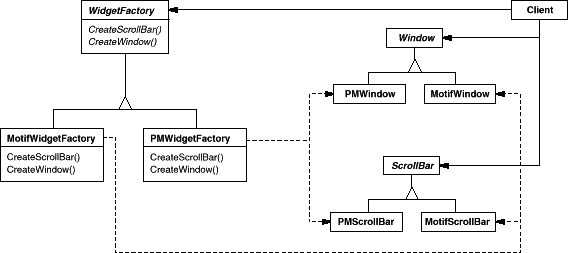
\includegraphics[width=.9\textwidth]{images/programovanie/abstractfactory1}

		\paragraph{Použiteľnosť}
		Návrhový vzor Abstract factory sa používa, ak:
			\begin{itemize}
				\item systém má byť nezávislý na tom, ako sú jeho produkty vytvárané
				\item systém má byť nakonfigurovaný s jednou z viacerých rodín produktov
				\item rodina príbuzných objektov produktov má byť používaná spolu a chceme pomôcť zabezpečiť toto obmedzenie
				\item chceme poskytovať knižnicu tried produktov, pričom chceme sprístupniť iba ich rozhrania a nie ich implementáciu
			\end{itemize}
		\paragraph{Štruktúra}

		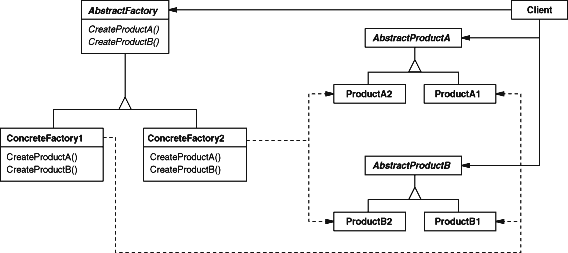
\includegraphics[width=.9\textwidth]{images/programovanie/abstractfactory2}

		\paragraph{Vzťahy (spolupráca)}
		Za normálnych okolností sa počas behu programu vytvára iba jediná všeobecne dostupná inštancia triedy AbstractFactory. Táto konkrétna továreň potom vytvára všetky komponenty (objekty majúce požadované správanie). Ak potrebujeme mať objekty viacerých typov, musíme si vytvoriť ďalšiu továreň (inštanciu indej triedy ConcreteFactory)\\
		AbstractFactory presúva vytváranie konkrétneho objektu na niektorú zo svojich odvodených tried ConcreteFactory.


		\paragraph{Dôsledky}:\\
		Návrhový vzor AbstractFactory má nasledovné výhody:
			\begin{itemize}
				\item Odstraňuje vytváranie konkrétnych tried z kódu aplikácie. Zodpovednosť za vytvorenie správneho typu objektu prenecháva AbstractFactory, pričom klient pracuje iba s abstraktnými rozhraniami a netrápi sa s konkrétnymi typmi.
				\item Dovoľuje jednoduchú výmenu rodín objektov. Keďže výber celej rodiny objektov je uskutočnený iba na jednom mieste, tam kde sa inicializuje AbstractFactory, dá sa tento výber ľahko zmeniť pomocou konfiguračného súboru. Dá sa však zmeniť aj počas behu programu. V našom prípade stačí vybrať novú ConcreteFactory a opätovne vytvoriť užívateľské rozhranie.
				\item Pomáha zvyšovať konzistenciu medzi produktami. Keď sú jednotlivé objekty rodín produktov navrhnuté tak, že majú fungovať spolu, je dôležité, aby boli používané naozaj iba objekty z jednej rodiny. Návrhový vzor AbstractFactory veľmi jednoducho túto podmienku zabezpečuje.
			\end{itemize}
		Návrhový vzor AbstractFactory má nasledovné nevýhody:
			\begin{itemize}
				\item Podpora nových typov produktov je zložitejšia. Ak by sme chceli pridať nový typ produktu (napr. SpecialButton), museli by sme zmeniť rozhranie triedy AbstractFactory a teda aj všetky triedy ConcreteFactory.
			\end{itemize}
		\paragraph{Implementácia}
			Ako sme už spomínali, je ťažšie pridávať nové typy produktov. Mohli by sme zmeniť návrh tak, že by sme pridali nový parameter do metód, ktoré vytvárajú objekty. Tento parameter by špecifikoval typ objektu (menu, tlačidlo, …), ktorý treba vytvoriť. Mohol by to byť identifikátor triedy, číslo, string alebo hocičo iné, čo by identifikovalo typ produktu. Potom by sme v triede AbstractFactory mali iba jednu metódu Make s parametrom určujúcim typ produktu. Takéto riešenie je jednoduchšie použiteľné v jazykoch bez striktnej typovej kontroly (napr. Smalltalk). V C++ môžeme toto riešenie použiť iba v prípade, ak všetky objekty majú spoločnú abstraktnú triedu (alebo môžu byť pretypované na jednu triedu). Objekt tejto triedy potom dostávame ako výsledok funkcie, čím vzniká problém, že nemáme prístupné metódy špecifické pre daný typ produktu. Preto ho musíme väčšinou pretypovať, čo zas nemusí byť bezpečné. Je to však cena za toto flexibilnejšie riešenie.

\section{Návrhové vzory: Bridge, Memento}


	\subsection{Bridge}
\paragraph{Účel}
Oddeliť abstrakciu od implementácie tak, aby sa mohli meniť nezávisle na sebe.

\paragraph{Ďalšie pomenovania}
Handle/Body

	\paragraph{Motivácia}:\\
		Keď má abstrakcia viacero možných implementácií, zvyčajná cesta, ako to naprogramovať je použitím dedenia. Abstraktná trieda definuje rozhranie a konkrétne podtriedy ju implementujú rôznymi spôsobmi. Tento prístup však nie je dostatočne flexibilný. Predstavme si implementáciu triedy Window, ktorú majú používať aplikácie, ktoré majú byť prenositeľné na viaceré oknové systémy (XWindow, Macintosh, …). Môžeme vytvoriť abstraktnú triedu Window a od nej pomocou dedenia odvodené triedy XWindow a MacWindow, ktoré implementujú danú triedu pre konkrétny systém. Toto riešenie má však nasledovné nevýhody:
		\begin{itemize}
			\item Ak by sme mali triedu IconWindow odvodenú od triedy Window, museli by sme urobiť pre ňu dve nové podtriedy XIconWindow a MacIconWindow. V konečnom dôsledku by sme museli vytvoriť jednu podtriedu pre každú dvojicu: typ systému, podtrieda triedy Window. Počet nových podtried by bol preto súčinom počtu podtried triedy Window a počtu systémov.\\

			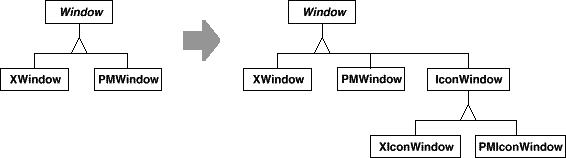
\includegraphics[width=.9\textwidth]{images/programovanie/bridge1}


			\item Zmena typu systému je príliš zložitá, keďže pri vytváraní okna už vytváram okno konkrétneho typu pre daný typ systému a zmena tohoto typu sa nedá jednoducho urobiť niekde na jednom mieste v kóde.
		\end{itemize}
		Návrhový vzor Bridge rieši tento problém oddelením hierarchií tried pre abstrakciu a implementáciu okna. Máme hierarchiu triedy Window (rôzne typy okien) a hierarchiu triedy WindowImp (implementácie pre rôzne oknové systémy).\\

	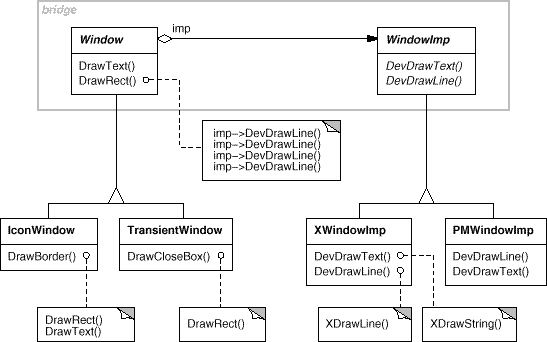
\includegraphics[width=.9\textwidth]{images/programovanie/bridge2}


		Všetky operácie na podtriedach triedy Window sú implementované pomocou abstraktných operácií definovaných v triede WindowImp. Tento návrhový vzor sa nazýva Bridge, lebo premosťuje abstrakciu a jej implementáciu, pričom sú však tieto dve hierarchie úplne nezávislé.

	\paragraph{Použiteľnosť}:\\
		Návrhový vzor Bridge sa používa, keď:
		\begin{itemize}
			\item chceme zabrániť pevnému prepojeniu medzi abstrakciou a implementáciou; napríklad ak chceme meniť implementáciu počas behu programu
			\item abstrakcia a aj implementácia majú byť nezávisle rozšíriteľné pomocou dedenia
			\item zmeny v implementácii nemajú mať vplyv na klienta, t.j. jeho kód sa nemusí prekompilovať
			\item chceme pred klientom kompletne schovať implementáciu
		\end{itemize}
	\paragraph{Štruktúra}:\\

		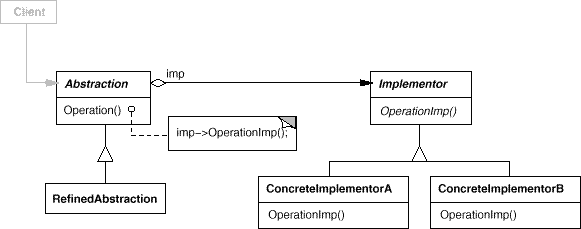
\includegraphics[width=.9\textwidth]{images/programovanie/bridge3}


	\paragraph{Účastníci}:
		\begin{enumerate}
			\item Abstraction (napríklad Window)\\
				deklaruje rozhranie abstrakcie; spravuje referenciu na objekt typu Implementor
			\item RefinedAbstraction (napríklad IconWindow)\\
				rozširuje rozhranie definované triedou Abstraction
			\item Implementor (napríklad WindowImp)\\
				Definuje rozhranie pre implementačné triedy. Toto rozhranie sa nemusí byť rovnaké ako rozhranie triedy Abstraction. Väčšinou toto rozhranie poskytuje iba primitívne operácie, zatiaľ čo rozhranie triedy Abstraction poskytuje operácie na vyššej úrovni.
			\item ConcreteImplementor (XWindowImp, MacWindowImp)\\
				Implementuje rozhranie triedy Implementor a definuje jeho konkrétnu implementáciu
		\end{enumerate}
	\paragraph{Vzťahy (spolupráca)}:
	Abstrakcia posiela požiadavky klienta príslušnému implementátorovi.

	\paragraph{Dôsledky}:\\
		Návrhový vzor Bridge má nasledovné dôsledky:
		\begin{itemize}
			\item Oddelenie abstrakcie a implementácie\\
			Implementácia nie je pevne zviazaná s abstrakciou a preto môže byť menená aj počas behu programu. Toto oddelenie zároveň eliminuje závislosti pri kompilovaní, preto nemusíme prekompilovať abstraktnú triedu ak sa zmenila implementácia. Navyše toto oddelenie prispieva k lepšej štruktúre systému.
			\item Zvýšená rozšíriteľnosť\\
			Môžeme nezávislo rozširovať hierarchie tried abstrakcie a implementácie.
			\item Ukrytie implementačných detailov pred klientom.
		\end{itemize}
	\paragraph{Implementácia}:\\
		Pri implementácii si treba uvedomiť viacero skutočností:
			\begin{itemize}
				\item Iba jeden ConcreteImplementor\\
				V situácii, keď bude iba jedna trieda ConcreteImplementor, nepotrebujeme abstraktnú triedu Implementor. Ide o degenerovaný prípad návrhového vzoru Bridge. Toto sa môže stať, ak chceme iba oddeliť implementáciu od abstrakcie, alebo chceme skryť nejaké implementačné záležitosti pred klientom.
				\item Vytvorenie správneho objektu Implementor.\\
				Kto vytvára objekt Implementor? Ak abstrakcia vie o všetkých triedach ConcreteImplementor, tak ho môže vytvárať sama. Takisto sa môže určiť preddefinovaná implementácia, ktorá sa potom môže meniť. Ďalšou možnosťu je prenechanie zodpovednosti inému objektu - definovanie AbstractFactory, ktorá bude vracať správnu implementáciu.
				\item Zdieľanie objektov Implementor.\\
				Jednotlivé objekty Implementor sa môžu zdielať, pričom sa uchováva počet referencií, ktoré naň odkazujú.
			\end{itemize}
	\subsection{Memento}
		\paragraph{Účel}
			Bez narušenia zapúzdrenia zachytiť a externe uchovať interný stav objektu tak, aby mohol byť tento objekt neskôr obnovený do tohto stavu.

		\paragraph{Ďalšie pomenovania}
			Token

		\paragraph{Motivácia}:\\
			\begin{itemize}
				\item Zapuzdrenie časti stavu objektov znemožňuje jeho externé uloženie.
				\item Porušenie zapuzdrenia narúša spoľahlivosť a rozšíriteľnosť.
			\end{itemize}
		\paragraph{Použiteľnosť}
			\begin{itemize}
				\item Keď je potrebné uložiť snímku stavu (alebo jeho časti) nejakého objektu tak, aby mohol byť tento stav neskôr obnovený.
				\item Keď priame rozhranie pre získanie stavu by zviditeľnilo implementačné detaily a narušilo zapuzdrenie objektu.
			\end{itemize}
		\paragraph{Štruktúra}:\\
			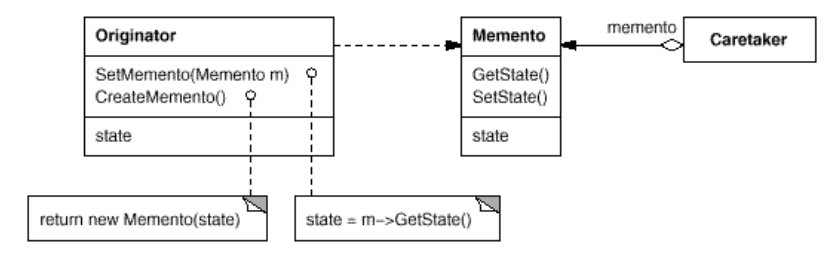
\includegraphics[width=.9\textwidth]{images/programovanie/memento1}

		\paragraph{Účastníci}:\\
			\begin{itemize}
			\item Memento\\
				Pamätá si interný stav objektu Originator\\
				Chráni stav pred prístupom od iného objektu ako originator
			\item Originator\\
				Vytvorí memento obsahujúce snímku jeho aktuálneho stavu\\
				Použije memento na obnovenie svojho stavu\\
				Používa široké rozhranie mementa
			\item Caretaker\\
				Zodpovedá za uloženie mementa\\
				Nikdy nepracuje s jeho obsahom\\
				Používa úzke rozhranie mementa
			\end{itemize}
		\paragraph{Vzťahy (spolupráca)}:\\

			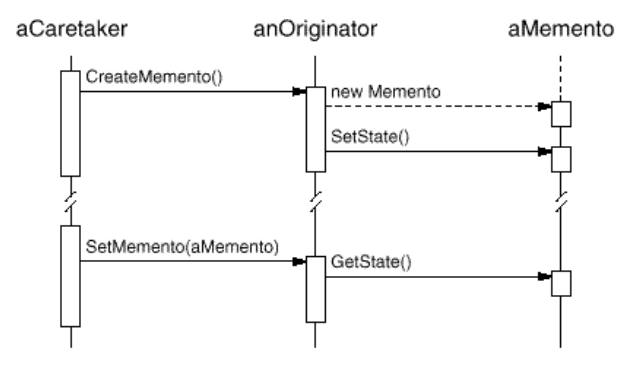
\includegraphics[width=.7\textwidth]{images/programovanie/memento2}
				\begin{enumerate}
				\item Caretaker\\
					Požaduje memento od originatora\\
					Nejaký čas si ho drží\\
					Pošle ho naspäť originátorovi, alebo ani nikdy nemusí
				\item Memento\\
					Je pasívne\\
					Iba originátor, ktorý ho vytvoril bude do neho zapisovať, alebo z neho čítať
				\end{enumerate}
		\paragraph{Dôsledky}
			\begin{itemize}
				\item Zachovanie hraníc zapúzdrenia
				\item Zjednodušuje originátora
				\item Používanie mement môže byť drahé, ak sa má kopírovať veľké množstvo pamäte
				\item Definovanie úzkeho a širokého rozhrania v niektorých jazykoch môže byť problém
				\item Skrytá cena starania sa o mementá - Caretaker nevie koľko informácie je v memente uložené
			\end{itemize}


\section{Návrhové vzory: Iterator, Visitor}

	\subsection{Iterator}
		\paragraph{Účel}
		Poskytuje spôsob, ako postupne pristupovať k prvkom štruktúry bez odkrytia vnútornej reprezentácie.
		\paragraph{Ďalšie pomenovania} Cursor (špecialný prípad)
		\paragraph{Motivácia}:\\
			Štruktúrované objekty (napr. listy) by nám mali poskytovať možnosť prístupu k ich prvkom bez exponovania vnútornej štruktúry. Navyše môžeme chcieť prechádzať štruktúrou rôznymi spôsobmi. Nechceme však príslušnú triedu zaplaviť množstvom metód na všetky možné spôsoby prechádzania, aké si len dokážeme vymyslieť (a možno by aj tak niekto chcel ešte iný spôsob). Riešením je vytvoriť nový objekt, ktorý prevezme zodpovednosť za prechod štruktúrou. Tento objekt si bude pamätať, v ktorých objektoch už bol. Trieda Iterator definuje rozhranie pre objekty zodpovedné za prechod štruktúrou.\\

			ListIterator bude zodpovedný za prechod štruktúrou List\\
				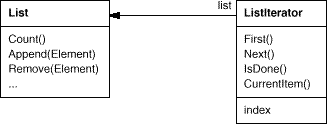
\includegraphics[width=.7\textwidth]{images/programovanie/iterator1}

			Konkrétny List, ktorým má prechádzať, sa poskytne objektu ListIterator už pri jeho vytváraní. Oddelením algoritmu na prechod štruktúrou od štruktúry môžeme jednoducho bez zasahovania do existujúceho kódu pridávať nové algoritmy. Všimnime si, že iterátor a list sú zviazané. T.j. klient pracuje s konkrétnym typom štruktúry. Radi by sme však zmenili typ štruktúry bez zmeny klientovho kódu. Majme napríklad SkipList, čo je štruktúra s vlastnosťami podobnými balancovaným stromom. Radi by sme vytvorili kód, ktorý bude schopný pracovať s oboma týmito štruktúrami. Definujeme si preto triedu AbstractList, ktorá poskytuje spoločné rozhranie pre manipuláciu s listami. Potom môžeme definovať podtriedy triedy Iterator pre každú podtriedu triedy AbstractList.\\

				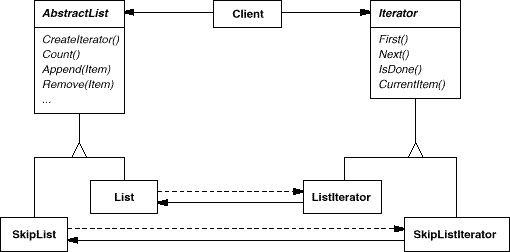
\includegraphics[width=.9\textwidth]{images/programovanie/iterator2}

			Pri vytváraní konkrétneho iterátora nám pomôže samotný list. V triede AbstractList si zadeklarujeme funkciu CreateIterator a necháme už na príslušné podtriedy, aby vytvorili iterátor vhodný pre ich štruktúru (hovoríme o polymorfickom iterátore).

			\paragraph{Použiteľnosť}:\\
			Návrhový vzor Iterator sa používa na:
				\begin{itemize}
					\item prístup k objektom zloženej štruktúry bez toho, aby sme sa zaoberali vnútornou reprezentáciu štruktúry
					\item podporu viacerých algoritmov na prechod štruktúrou
					\item poskytnutie jednotného rozhrania na prechádzanie rôznymi typmi štruktúr
				\end{itemize}
			\paragraph{Štruktúra}:\\

				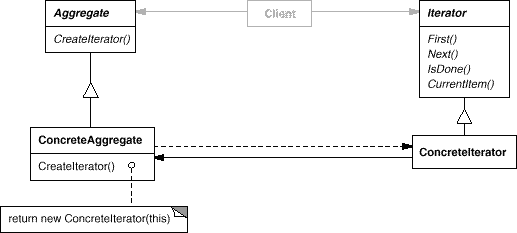
\includegraphics[width=.9\textwidth]{images/programovanie/iterator3}

			\paragraph{Účastníci}:\\
				\begin{enumerate}
					\item Iterator\\
						definuje rozhranie pre prechod štruktúrou
					\item ConcreteIterator\\
						Implementuje rozhranie triedy Iterator\\
						Uchováva si aktuálnu pozíciu počas prechodu štruktúrou
					\item Aggregate\\
						definuje rozhranie pre vytvorenie objektu Iterator
					\item ConcreteAggregate\\
					implementuje funkciu na vytvorenie konkrétneho objektu ConcreteIterator
				\end{enumerate}
			\paragraph{Vzťahy (spolupráca)}:\
				Objekt ConcreteIterator prechádza dokumentom, pričom vie, ktorý je aktuálny prvok a vie vypočítať nasledujúci prvok.
			\paragraph{Dôsledky}
				Návrhový vzor Iterator má nasledovné dôsledky:
				\begin{enumerate}
					\item Poskytuje možnosť jednoduchého zmenenia spôsobu prechodu štruktúrou.
					\item Iterator zjednodušuje rozhranie triedy Aggregate (lebo metódy na prechod štruktúrou sú vybrané preč).
					\item Jedna štruktúra môže byť prechádzaná viacerými iterátormi naraz v tom istom čase.
				\end{enumerate}
			\paragraph{Implementácia}:\\

			Iterator má veľa variant a alternatív. Niektoré programovacie jazyky priamopodporujú niektoré z nich.
			\begin{enumerate}
				\item Kto kontroluje prechod? Základným problémom je, či prechod štruktúrou kontroluje klient - vtedy ide o externý iterátor, alebo ho kontroluje iterátor sám - vtedy ide o interný iterátor. Pri externých iterátoroch si klient pýta aktuálny prvok a pomocou operácie Next (alebo podobnej) sa posúva na ďalší prvok. Pri interných iterátoroch sa iterátoru odovzdá operácia a on už sám prechádza štruktúrou a vykonáva danú operáciu. V jazykoch, ktoré nepodporujú anonymné funkcie (napr. C++) vzniká problém s implementáciou interných iterátorov. Externé iterátory sú navyše flexibilnejšie, hoci interné iterátory sú zasa jednoduchšie (na niektoré problémy v niektorých jazykoch).
				\item Kto definuje prechodový algoritmus? Iterator nie je jediným miestom, kde môže byť definovaný algoritmus prechodu. Môže byť definovaný aj v triede Aggregate a Iterator sa použije iba na uchovanie stavu iterácie. Vtedy hovoríme iterátoru aj Cursor. Klient potom volá operáciu Next na objekte Aggregate, pričom Cursor je argument. Operáciu Next mení stav objektu Cursor. Tento spôsob môže byť užitočný, ak iterátor používa privátne premenné objektu Aggregate, ktoré nechceme (alebo nemôžeme) zprístupniť.
				\item Ako robustná je iterácia? Ak počas prechodu štruktúrou túto štruktúru meníme (pridávame alebo mažeme prvky), môže sa stať, že niektorý prvok vynecháme alebo prejdeme viackrát, prípadne sa zacyklíme. Jednoduchým riešením by bolo zkopírovať celú štruktúru a prechádzať kópiou, je to však vo všeobecnosti príliš drahé. Je viacero spôsobov, ako zabezpečiť, aby bol iterátor robustný (t.j. prešiel správne štruktúrou aj ak sa bude meniť). Môže napríklad Aggregate pri každom pridávaní a mazaní prvkov prispôsob vnútorný stav iterátorov, ktoré vytvoril, alebo si potrebnú informáciu ukladá u seba.
				\item Prídavné operácie iterátora. Medzi základné operácie iterátora patria: First, Next, IsDone, CurrentItem. Avšak aj niektoré ďaľšie môžu mať svoj význam (napr. Previos, SkipTo).
				\item Iterátory môžu mať privilegovaný prístup. Na iterátor môžeme pozerať ako na rozšírenie objektu Aggregate, ktorý ho vytvoril. Iterator a Aggregate sú úzko zviazané. Môžeme preto triedu Iterator definovať ako zpriatelenú(friend) triedu triedy Aggregate.
				\item Iterátory pre kompozitné objekty.
				\item Null iterátor. NullIterator je degenerovaný iterátor, ktorý sa používa pre ošetrenie hraničných hodnôt. Jeho funkcia IsDone vracia vždy true, čo vlastne znamená, že už prešiel všetkými svojimi deťmi. NullIterator je používaný napríklad v listoch stromu, čím nám umožňuje jednotný prístup na prechádzanie štruktúrou.
			\end{enumerate}


	\subsection{Visitor}
		\paragraph{Účel}
			Reprezentuje operáciu, ktorá má byť vykonaná na prvkoch štruktúry. Visitor nám dovoľuje definovať nové operácie bez zmeny tried elementov, na ktorých majú byť vykonané.
		\paragraph{Motivácia}
		Majme kompilátor, ktorý reprezentuje programy pomocou abstraktných syntaktických stromov. Potrebuje vykonávať operácie statickej analýzy, ako napr. kontrola, či sú všetky premenné definované, či je premennej priradená hodnota skôr, ako je použitá, kontrola typov, optimalizácia kódu, … Navyše môže využívať syntaktické stromy na krajšie zobrazenie programu (odsadenie, …), počítanie rôznych metrík, … Väčšina z týchto operácii potrebuje, aby sa k jednotlivým typom uzlov pristupovalo rôzne (t.j. inak sa správať k priradeniu, inak k uzlom reprezentujúcim premenné, aritmetické výrazy, …) . Na obrázku je časť hierarchie triedy Node.\\


			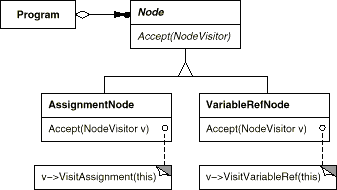
\includegraphics[width=.7\textwidth]{images/programovanie/visitor1}

		Problémom je, že tým, že všetky operácie budeme implementovať vo všetkych podtriedach triedy Node, dostaneme kód, ktorý je veľmi ťažko zrozumiteľný, ťažko sa udržiava a mení.Je to spôsobené tým, že metódy jednotlivých operácií sú pomiešané a vznikajú dlhé a neprehľadné triedy. Navyše pridanie novej triedy zvyčajne vyžaduje prekompilovanie všetkých tried. Bolo by lepšie, keby sa nová operácia mohla pridať bez toho, aby sa robili zmeny v triede Node a v jej podtriedach. Obe tieto požiadavky môžeme splniť tak, že jednotlivé operácie zapúzdrime do samostatného objektu nazvaného Visitor, ktorý budeme poskytovať uzlom syntaktického stromu, keď ním budeme prechádzať. Keď uzol 'akceptuje' daný objekt Visitor (t.j. v metóde Accept), pošle požiadavku objektu Visitor, v ktorej je zašiforvaný aj typ uzla. Navyše obsahuje daný uzol ako parameter. Objekt Visitor potom vykoná operáciu pre daný typ objektu. Napríklad kompilátor, ktorý by nepoužíval objekt Visitor by mohol kontrolu typov implementovať pomocou metódy TypeCheck na uzloch syntaktického stromu. Ak by kompilátor používal návrhový vzor Visitor, vytvoril by objekt TypeCheckingVisitor a volal by metódu Accept na uzloch syntaktického stromu. Argumentom metódy Accept by bol práve TypeCheckingVisitor. Každá trieda odvodená od triedy Node by v metóde Accept volala naspäť metódu objektu TypeCheckingVisitor, ktorá je priradená danému typu uzla. Napríklad trieda VariableRefNode by volala metódu VisitVariableRef. To, čo zvyklo byť naimplementované v metóde TypeCheck v triede VariableRefNode bude teraz naimplementované v metóde VisitVariableRef v triede TypeCheckingVisitor. Aby sme nezostali iba pri kontrole typov, pridáme abstraktnú triedu NodeVisitor, ktorú potom budeme môcť používať aj na ostatné analýzy. Trieda NodeVisitor bude musieť deklarovať metódu pre každú triedu odvodenú od triedy Node. Pre nové typy analýzy už len odvodíme novú triedu od triedy NodeVisitor a nemusíme meniť existujúce triedy.\\


		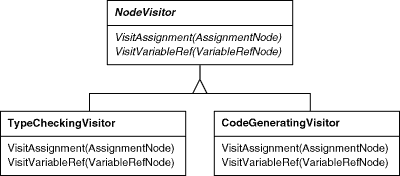
\includegraphics[width=.7\textwidth]{images/programovanie/visitor2}






		Návrhový vzor Visitor definuje dve hierarchie tried. Jednu pre objekty, na ktorých sa operácie vykonávajú (hierarchia Node) a druhú pre objekty, ktoré definujú operácie na týchto objektoch (hierarchia NodeVisitor).

		\paragraph{Použiteľnosť}:\\
		Návrhový vzor Visitor sa používa, keď:
			\begin{itemize}
				\item máme štruktúru objektov, ktorá obsahuje veľa rôznych tried objektov s rozdielnym rozhraním, pričom chceme vykonávať operácie na týchto objektoch, ktoré závisia od typu objektu.
				\item veľa rôznych a navzájom nesúvisiacich operácií sa má vykonať na objektoch v štruktúre objektov, pričom však nechceme, aby sme triedy týchto objektov 'zneprehľadnili' týmito operáciami.
				\item triedy reprezentujúce štruktúru objektov sa menia iba veľmi zriedkavo, alo často chceme definovať nové operácie nad touto štruktúrou
			\end{itemize}
		\paragraph{Štruktúra}:\\
			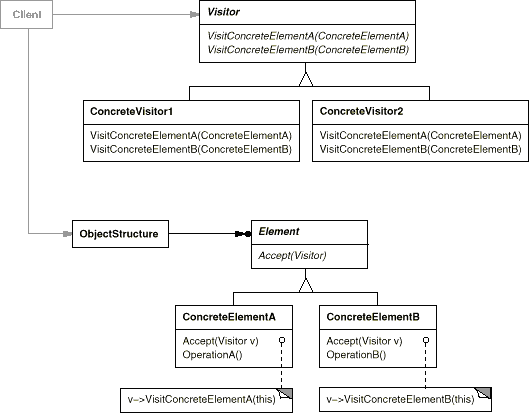
\includegraphics[width=.9\textwidth]{images/programovanie/visitor3}

			\begin{enumerate}
				\item Visitor (NodeVisitor)\\
					deklaruje operáciu Visit pre každú triedu ConcreteClass v štruktúre objektov. Meno operácie a jej argumenty určujú triedu, ktorá posiela požiadavku Visit triede Visitor.
				\item ConcreteVisitor (TypeCheckingVisitor)\\
					implementuje každú operáciu Visit deklarovanú v triede Visitor.
				\item Element (Node)\\
					deklaruje operáciu Accept, ktorá má ako argument triedu Visitor.
				\item ConcreteElement (VariableRefNode)\\
					implemenuje operáciu Accept.
				\item ObjectStructure (Program)\\
					vie vymenovať svoje elementy\\
					môže poskytovať 'vysoko-úrovňové rozhranie' na prístup k svojim elementom\\
					môže byť objektom typu Composite, alebo kolekcia typu list, množina, …
			\end{enumerate}

		\paragraph{Vzťahy (spolupráca)}:\\
			\begin{itemize}
				\item Klient, ktorý používa návrhový vzor Visitor musí vytvoriť objekt ConcreteVisitor a potom prechádzať štruktúrou objektov, pričom každý element navštívi s objektom Visitor.
				\item Keď je element navštívený, volá operáciu triedy Visitor, ktorá prislúcha jeho triede. Daný element poskytne sám seba ako argument tejto operácie, aby Visitor mohol pristupovať k jeho stavu, ak je to potrebné.
			\end{itemize}
			Na obrázku je znázornená spolupráca medzi štruktúrou objektov, objektom Visitor a dvoma elementami.\\


			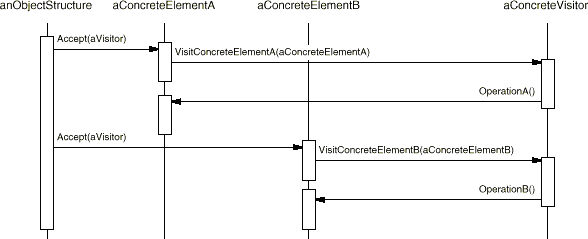
\includegraphics[width=.9\textwidth]{images/programovanie/visitor4}

		\paragraph{Dôsledky}:\\
			Návrhový vzor Visitor má nasledovné výhody a nevýhody:
			\begin{enumerate}
			\item Jednoduché pridanie novej operácie\\
				Pri pridávaní novej operácie nemusíme zasahovať do tried reprezentujúcich štruktúru, ale iba vytvoríme novú podtriedu triedy Visitor.
			\item Združuje príbuzné operácie a oddeľuje nesúvisiace\\
				Metódy vykonávajúce jednu operáciu nie sú roztrúsené v triedach reprezentujúce štruktúru, ale sú sústredené v objekte Visitor. Naopak, metódy vykonávajúce rôzne operácie sú oddelené tým, že sú každá v inej triede odvodenej od triedy Visitor. Navyše všetky dáta špecifické pre nejaký algoritmus môžu byť ukryté v objekte Visitor.
			\item Pridanie novej triedy ConcreteElement je zložitejšie\\
				Ak chceme pridať novú podtriedu triedy Element (Node), musíme pridať novú metódu do triedy Visitor a teda aj do každej triedy ConcreteVisitor. Ak by sme v triede Visitor definovali preddefinované správanie, nemuseli by sme meniť každú triedu ConcreteVisitor, avšak vo väčšine prípadov sa takéto preddefinované správanie dá uplatniť iba na nepatrné percento tried.
			\item Prechádzanie hierarchiami tried\\
				Na prechádzanie štruktúrou objektov môže byť použitý objekt Iterator. Objekt Iterator má obmedzenie v tom, že jednotlivé elementy musia mať spoločnú abstraktnú triedu. Objekt Visitor toto obmedzenie nemá, keďže si môžeme zadefinovať operáciu Visit pre ľubovoľný typ objektu.
			\item Akumulovanie stavu\\
				Objekt Visitor môže pri prechádzaní štruktúrou akumulovať stav. Bez tohoto objektu by sme si museli stav odovzdávať pomocou argumentov, alebo by bol uložený v globálnych premenných.
			\item Porušenie zapúzdrenia\\
				Návrhový vzor Visitor predpokladá, že rozhranie triedy ConcreteElement poskytuje dostatok informácie na to, aby mohol objekt Visitor vykonávať svoju činnosť. To častokrát speje k tomu, že ConcreteElement poskytuje vo svojom rozhraní prístup k svojmu vnútornému stavu, čo môže kompromitovať zapúzdrenie.
				\end{enumerate}
		\paragraph{Implementácia}:\\
			Pri implementácii si treba uvedomiť viacero faktov:
			\begin{enumerate}
				\item Double dispatch\\
				Návrhový vzor Visitor používa techniku double-dispatch. Túto techniku priamo používajú niektoré jazyky (napr. CLOS). Jazyk C++ podporuje single-dispatch. V jazykoch podporujúcich single-dispatch určujú operáciu, ktorá bude vykonaná dve kritéria: meno operácie a typ prijímateľa. Double-dispatch jednoducho znamená, že operácia, ktorá bude vykonaná závisí od mena operácie a dvoch typov prijímateľov. Napríklad Accept závisí od typu dvoch objektov: Visitor a Element.
				\item Kto je zodpovedný za prechod štruktúrou? Zodpovednosť za prechod štruktúrou môžeme umiestniť na tri miesta:\\
					do štruktúry objektov (ak máme napríklad kolekciu)\\
					do objektu Visitor\\
					do samostatného objektu Iterator
			\end{enumerate}
